\documentclass[11pt, letterpaper]{article}
\usepackage[utf8]{inputenc}

\usepackage[margin=1in]{geometry}

\usepackage{amsmath,amsfonts,amssymb,amsthm,pgf,tikz,enumerate,xcolor,graphicx,microtype}
\usepackage[colorlinks]{hyperref}

\theoremstyle{definition}
\newtheorem{defn}{Definition}
\newtheorem{ex}{Example}

\theoremstyle{remark}
\newtheorem*{rmk}{Remark}

\begin{document}

\begin{center}
{\Large {\sc MATH 1077 -- Exploring Modern Mathematics}}
\\[1em]
{\large Fall 2024}
\end{center}

\begin{center}
	\rule{6in}{0.4pt}
	\\[2pt]
	\begin{tabular}{llcll}
		{\bf Instructor:} &Taylor Dupuy &\quad &	{\bf Email:}&\href{mailto:taylor.dupuy@gmail.com}{taylor.dupuy@gmail.com} \\
		{\bf Section A:} &MWF 9:40am -- 10:30am &\quad &{\bf Section B:} &MWF 10:50am -- 11:40am \\
		{\bf Place:} &ROWELL HLTH 110 &\quad &{\bf Place:} &ROWELL HLTH 111 \\
	\end{tabular}
	\rule{6in}{0.4pt}
\end{center}

\vspace{2em}

\noindent {\bf Office hours:} Innovation 439,TBD
\vspace{1em}

\noindent {\bf Course webpage:} \url{https://tdupu.github.io}
\vspace{1em}

\noindent {\bf Description and objectives:} 
We examine various subjects not typically seen in traditional math courses. Topics may  include but are not limited to, the mathematics of the 2009 mayoral election in Burlington (and how it relates to slime molds),  how to win on a game show, why coin-flipping is deep, how to cross every bridge in a city with many bridges exactly once, how a group of students at MIT beat the lottery (and how to win at poker), why money is worth less to rich people, and symmetry (and the golden ratio).

\par 
The most important thing for me is for people to come away from this class with a broader understanding of what mathematical thinking really is.

\vspace{1em}

\noindent {\bf Books:} 
\begin{itemize}
\item (main) {\it Excursions in Modern Mathematics} by Peter Tannenbaum (10th Edition).

The book \emph{Excursions in Mathematics} can be both dry and terse which is not ideal for this course emphasizing ideas. 
I did not select this book. 
To make up for this, I'm going to supplement.

\item (supplement) \emph{The Magic Of Mathematics} by Gross and Harris. 
You do not need to buy this book. The chapters you may want to read are on the course webpage. They are limited to counting and probability.

\item (supplement) \emph{How Not To Be Wrong} by Ellenberg. 
You do not need to buy this book. I learned many of the stories I'm going to tell from this book and wanted to cite it here.
\end{itemize}



\vspace{1em}


\noindent {\bf Technology:} No special technology is needed. 
No blackboard. 
No online homework. 
In the rare event that we move online due to an unforeseen COVID surge we will meet on MSTeams.
\vspace{1em}



\noindent {\bf Types of assignments}

\begin{itemize}
	\item {\bf Reflections}: These are written assignments due at the beginning of a class assigned during a previous class. 
	They are credit/no-credit and to get full credit one needs to just needs to participate in the reflection (while short responses are acceptable, single sentences scribbled before class having nothing to do with the reflection don't count). 
	Before introducing a new idea I will assign a reflection which will facilitate a discussion to follow in a later period. 
	They are typically of the form ``try $X$'' or ``what do you think about $X$?''.
	\item {\bf Homework}: Homework problems accompanying class discussions can be found on the course webpage. Although they will not be collected in full, there will be periodic zzes over the homework problems which will either be identical to or very similar to the homework problems.
	\item {\bf Quizzes}: We will give in-class quizzes for every homework assignment. Quizzes are open book, open note, and open calculator so students are encouraged to work out all of the homework questions in advance to improve their scores.
	\item {\bf Quiz Redo}: There will be two ``quiz redo'' sessions which serve as the midterm and final respectively. 
	Each exam is an opportunity to replace quiz scores with ones that were previously missed.
\end{itemize}

\noindent {\bf Grading}
Grades will be based on quizzes and reflections each contributing equal weight.
\begin{itemize}
\item {\em Quizzes and reflections (100\%)} recognizing that everyone will miss quizzes or reflections from time to time we allow for \emph{three omissions of quizzes and reflections}. 
\item {\em Quiz Redos } 
In addition to dropping quizzes, we allow students to replace all the quizzes for a given ``period'' with during a midterm quiz-redo session and a final quiz-redo session. 
\end{itemize}

\noindent Final letter grades are assigned according to the following table.
\begin{center}
	\begin{tabular}{ |c|c|c|c|c|c| }
		\hline
		A+ & 97-100 & A & 93-96 & A- & 90-92 \\ 
		\hline
		B+ & 87-89 & B & 83-86 & B- & 80-82 \\ 
		\hline
		C+ & 77-79 & C & 73-76 & C- & 70-72 \\ 
		\hline
		D+ & 67-69 & D & 63-66 & D- & 60-62 \\ 
		\hline
		F & $< 60$ &&&& \\
		\hline 
	\end{tabular}
\end{center}
\vspace{1em}




\noindent {\bf Important dates:} 
\begin{center} 
	\begin{minipage}{3.8in}
		\begin{flushleft}
			Labor Day Holiday \dotfill ~Sep 2 \\
			Add/Drop, Pass/No Pass, Audit Deadline \dotfill ~Sep 9 \\
			Fall Recess \dotfill ~Oct 11 \\
			Last Day to Withdraw \dotfill ~Oct 28 \\
			Thanksgiving Recess \dotfill ~Nov 25-29 \\
			Last Day of Classes \dotfill ~Dec 6 \\
		\end{flushleft}
	\end{minipage}
\end{center}
\vspace{1em}

\noindent {\bf Final Exam Schedule:} 
\begin{itemize}

\item	\textbf{MATH 1077 A (Exploring Modern Mathematics)} \\
	Date: 12-DEC-2024 \\
	Time: 10:30 am - 1:15 pm \\
	Location: ROWELL 110 \\
	
	\item \textbf{MATH 1077 B (Exploring Modern Mathematics)} \\
	Date: 13-DEC-2024 \\
	Time: 7:30 am - 10:15 am \\
	Location: ROWELL 111 \\
\end{itemize}
\vspace{1em}

\noindent {\bf Math help sessions} 
UVM Mathematics PhD students hold math help sessions every weekday starting around 5PM and ending around 7PM. 
I would recommend visiting those help sessions for assistance as our gradaute students are excellent.
These are located on the 4th floor of the Innovation building every weekday. Please check the Mathematics and Statistics Department webpage for scheduling details. 

\vspace{1em}

\noindent {\bf Expectations:} Students are expected to regularly attend class, complete any assigned work, and comply with UVM's \href{http://www.uvm.edu/policies/student/studentcode.pdf}{{\em Code of Student Conduct}}.
Moreover, students are expected to act with {\em academic integrity}. That is, the student may not plagiarize or fabricate any work, nor may the student collude or cheat. See UVM's \href{https://www.uvm.edu/policies/student/acadintegrity.pdf}{{\em Code of Academic Integrity}}.
\vspace{1em}

\noindent {\bf ADHD statement} I have combined type ADHD. 
This sometimes manifests itself in typos and oversights in my first time teaching a course (this is my first time teaching this class). 
If you find any mistakes or I forget to respond to something give me a nudge.
I thank you in advance for your patience.

\noindent {\bf Student learning accomodations:} In keeping with University policy, any student with a documented disability interested in utilizing ADA accommodations should contact Student Accessibility Services (SAS), the office of Disability Services on campus for students. SAS works with students and faculty in an interactive process to explore reasonable and appropriate accommodations, which are communicated to faculty in an accommodation letter. All students are strongly recommended to discuss with their faculty the accommodations they plan to use in each course. Faculty who receive Letters of Accommodation with Disability Related Flexible accommodations will need to fill out the Disability Related Flexibility Agreement. Any questions from faculty or students on the agreement should be directed to the SAS specialist who is indicated on the letter. 
\begin{tabular}{ll}
{\em Contact SAS:} &A170 Living/Learning Center; \\
&802-656-7753 \\ 
&\href{mailto:access@uvm.edu}{access@uvm.edu} \\
&\href{https://www.uvm.edu/access}{www.uvm.edu/access}
\end{tabular}

\vspace{1em}

\noindent {\bf Religious holidays} Students have the right to practice the religion of their choice. If you need to miss class to observe a religious holiday, please submit the dates of your absence to me in writing by the end of the second full week of classes. You will be permitted to make up work within a mutually agreed-upon time. See \href{https://www.uvm.edu/registrar/religious-holidays}{www.uvm.edu/registrar/religious-holidays}.
\vspace{1em}

\noindent {\bf FERPA rights disclosure:} The purpose of this policy is to communicate the rights of students regarding access to, and privacy of their student educational records as provided for in the Family Educational Rights and Privacy Act (FERPA) of 1974. See \href{http://catalogue.uvm.edu/undergraduate/academicinfo/ferparightsdisclosure/}{here} for the disclosure.
Sensitive emails should be sent to \href{mailto:tdupuy@uvm.edu}{tdupuy@uvm.edu}.
\vspace{1em}

\noindent {\bf Promoting health and safety:} \\
{\em Center for Health and Wellbeing}:
\url{https://www.uvm.edu/health} \\
{\em Counseling \& Psychiatry Services} (CAPS):
Phone: (802) 656-3340 \\
{\em C.A.R.E.}: If you are concerned about a UVM community member or are concerned about a specific event, we encourage you to contact the Dean of Students Office (802-656-3380).  If you would like to remain anonymous, you can report your concerns online by visiting the Dean of Students website at \url{https://www.uvm.edu/studentaffairs}
\vspace{1em}

\iffalse 
\begin{figure}
\centering
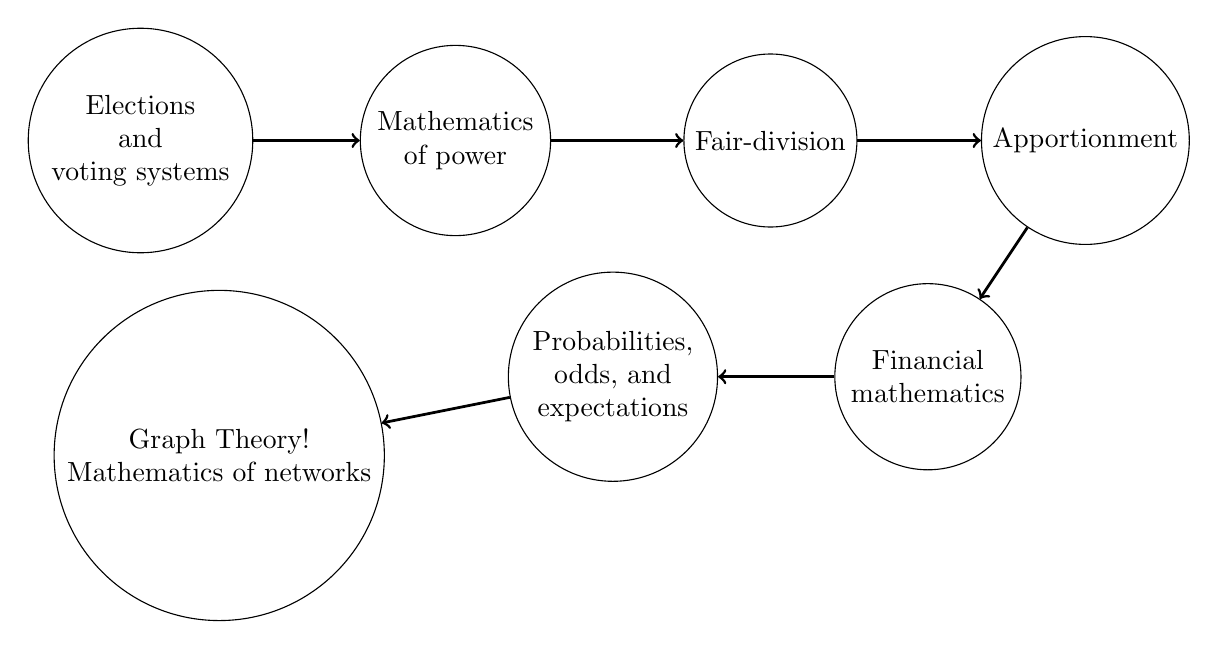
\begin{tikzpicture}
[node/.style={circle, draw=black!100}]

\node[node] (1) at (0,0) [draw, align=center] {Elections \\ and \\ voting systems};
\node[node] (2) at (4,0) [draw, align=center] {Mathematics \\ of power};
\node[node] (3) at (8,0) [draw, align=center] {Fair-division};
\node[node] (4) at (12,0) [draw, align=center] {Apportionment};
\node[node] (5) at (10,-3) [draw, align=center] {Financial \\ mathematics};
\node[node] (6) at (6,-3) [draw, align=center] {Probabilities, \\ odds, and \\ expectations};
\node[node] (7) at (1,-4) [draw, align=center] {Graph Theory! \\ Mathematics of networks};

\draw[->, line width=1pt] (1) edge (2);
\draw[->, line width=1pt] (2) edge (3);
\draw[->, line width=1pt] (3) edge (4);
\draw[->, line width=1pt] (4) edge (5);
\draw[->, line width=1pt] (5) edge (6);
\draw[->, line width=1pt] (6) edge (7);
\end{tikzpicture}
\caption{Math017, a Hamilton path.}
\label{fig:math17hamiltonpath}
\end{figure}
\fi



\end{document}